\section*{ПРИЛОЖЕНИЕ A}\label{sec:app-A}
\addcontentsline{toc}{section}{ПРИЛОЖЕНИЕ A}

\lstinputlisting
[
    basicstyle=\tiny,
    caption = Дополненная грамматика языка tinyc \label{lst:grammar}
]
{code/full_tinyc.g4}
\pagebreak

\section*{ПРИЛОЖЕНИЕ Б}\label{sec:app-B}
\addcontentsline{toc}{section}{ПРИЛОЖЕНИЕ Б}
\begin{figure}[h!]
	\begin{center}
		{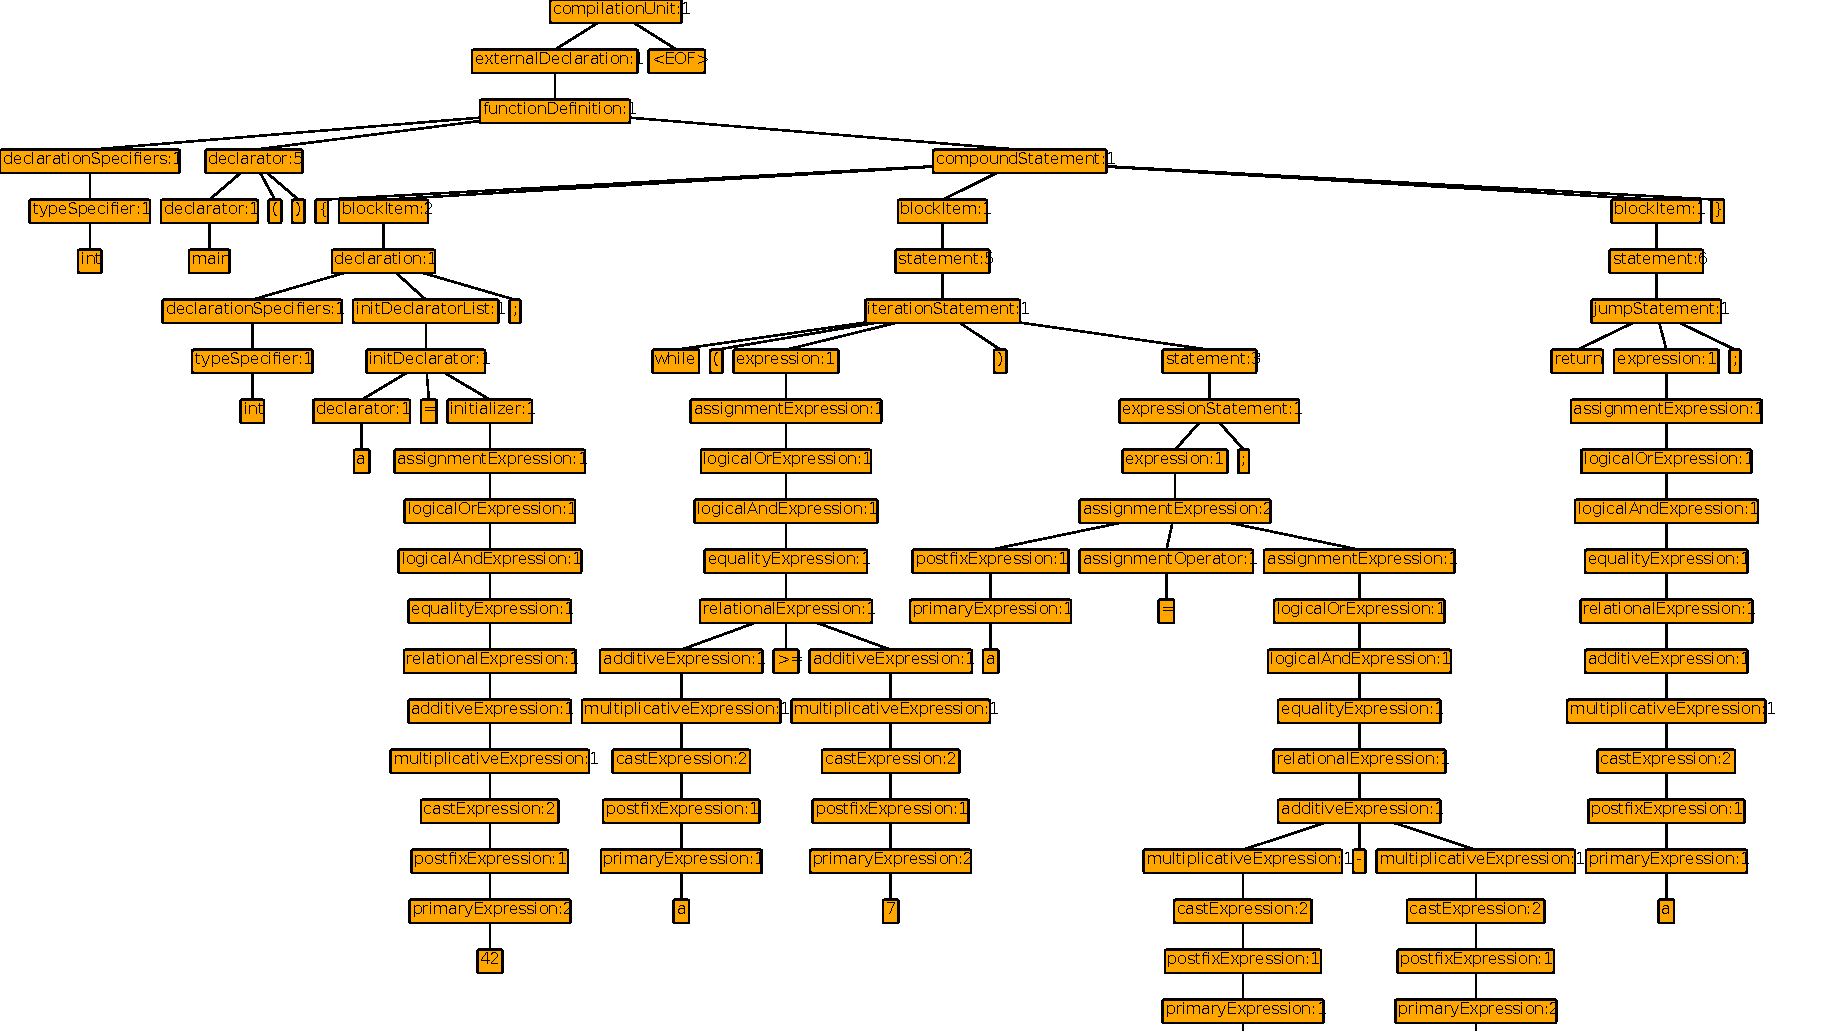
\includegraphics[width=0.85\textheight, angle = 90]{img/div7.pdf}}
		\caption{Пример визуализации синтаксического дерева.}
		\label{div7:tree}
	\end{center}
\end{figure}
